\subsubsection{Dataset}
\label{sec:dataset}

The data come from a traffic-imagery release published by Peru's Ministry of Transportation and Communications (MTC)~\cite{MTC2026SmartChallenge}. The task is oriented vehicle detection and classification with rotated boxes, which means that each predicted vehicle must include both category and geometry. In this study, the original archives and CSV annotations are treated as external inputs consumed by preprocessing scripts and not redistributed in the repository. Table~\ref{tab:dataset_structure} summarizes the files used by the workflow and separates the role of training frames, held-out frames, public annotations, and submission templates.

\begin{table*}[!t]
  \caption{MTC traffic-imagery data files and their role in the workflow.}
  \label{tab:dataset_structure}
  \centering
  \small
  \begin{tabular}{p{0.20\textwidth} p{0.12\textwidth} p{0.16\textwidth} p{0.42\textwidth}}
    \toprule
    \textbf{Item} & \textbf{Size} & \textbf{Rows / Images} & \textbf{Role} \\
    \midrule
    \texttt{train.zip} & 40.3 GB & 54,262 images & Training frames used to create resized images, YOLO-OBB labels, split metadata, pseudo-labels, and augmentation sources. \\
    \texttt{test.zip} & 17.3 GB & 23,579 images & Held-out frames without public labels; not used for local validation metrics. \\
    \texttt{train.csv} & 19.4 MB & 54,262 rows & Public training annotations stored as \texttt{Id} and \texttt{Target} columns. \\
    \texttt{sample\_submission.csv} & 552.6 KB & 23,579 rows & Submission template with \texttt{Target} initialized to \texttt{none}. \\
    \bottomrule
  \end{tabular}
\end{table*}

Each object record contains a category identifier, center coordinates, width, height, and an angle in degrees. Frames with multiple vehicles store records separated by semicolons, whereas frames without annotated moving vehicles use the literal value \texttt{none}. The preprocessing stage converts these parametric OBB annotations into YOLO-OBB corner coordinates and remaps the official class identifiers from 1--9 to the zero-indexed labels required for training. This conversion is necessary because the training pipeline expects one label file per image and one line per object, with the class identifier followed by eight normalized corner coordinates.

Frame identifiers follow the pattern \texttt{v\_[clip]\_[frame]}, where the final number marks the temporal position within a short clip. This organization is central to the split design because adjacent frames share viewpoint, background, and illumination. If individual frames were split randomly, near-duplicate visual evidence from the same clip could appear in both training and validation. To avoid this leakage, the preprocessing pipeline assigns complete clips, rather than individual frames, to a single split. Table~\ref{tab:clip_statistics} reports the resulting clip statistics.

\begin{table}[!t]
  \caption{Per-split clip statistics derived from frame identifiers.}
  \label{tab:clip_statistics}
  \centering
  \small
  \begin{tabular}{lrr}
    \toprule
    \textbf{Statistic} & \textbf{Train} & \textbf{Test} \\
    \midrule
    Number of clips & 1,088 & 473 \\
    Minimum frames per clip & 18 & 23 \\
    Mean frames per clip & 49.87 & 49.85 \\
    Median frames per clip & 50 & 50 \\
    Maximum frames per clip & 50 & 50 \\
    \bottomrule
  \end{tabular}
\end{table}

The dataset defines nine vehicle categories. Some categories with similar shape and scale, such as combi, microbus, and minibus, are visually difficult to separate from elevated viewpoints, so class ambiguity must be considered during interpretation. The analysis code verifies that class identifiers remain within range, dimensions stay positive, centers fall inside the frame, and angles follow the expected convention. Figure~\ref{fig:dataset_obb_sample} illustrates the rotated annotation format used by the task and shows why OBB geometry is preferable to horizontal boxes in dense traffic frames.

\begin{figure}[!t]
  \centering
  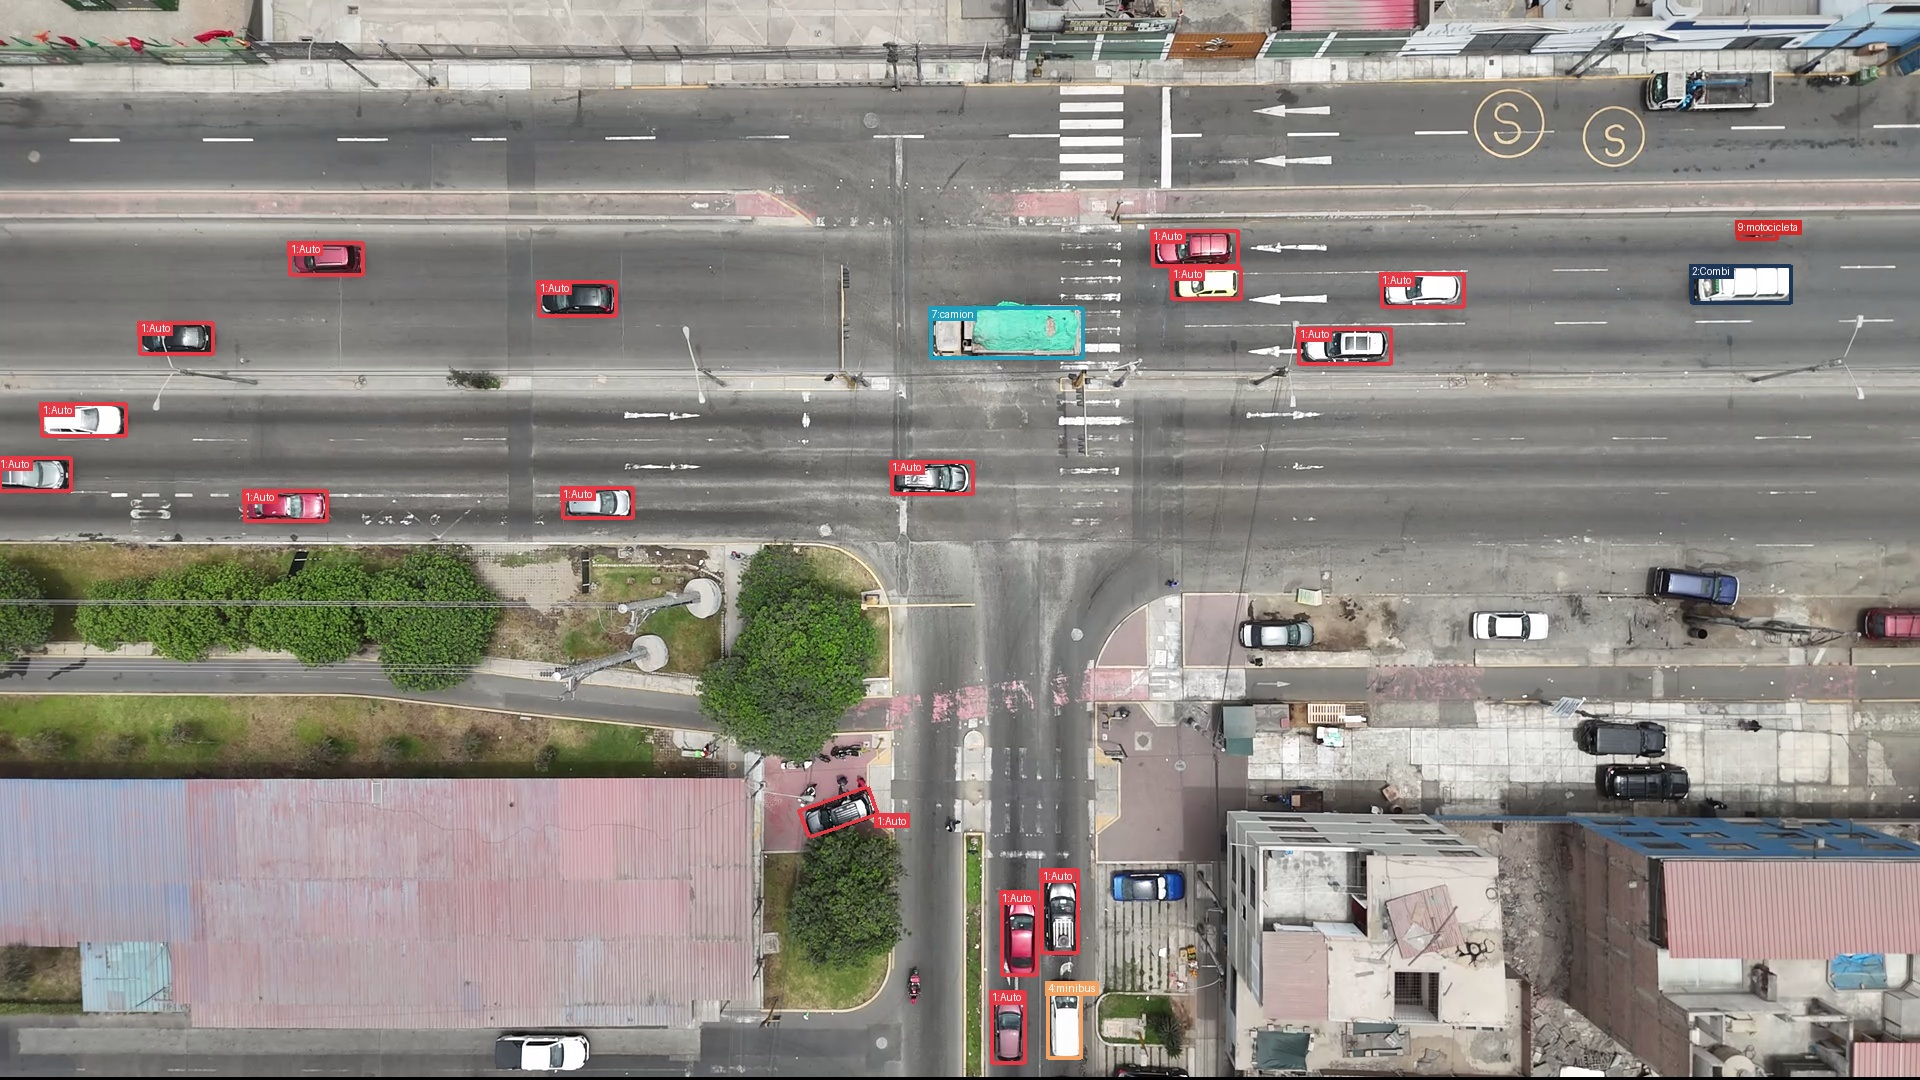
\includegraphics[width=\columnwidth]{latex_report/src/fig/dataset_obb_sample.jpg}
  \caption{Representative oriented bounding box annotations in a traffic frame.}
  \label{fig:dataset_obb_sample}
\end{figure}

The statistical audit identified 601,934 annotated objects across 54,262 training frames. Among these frames, 3,394 contain no annotated objects, 6,212 contain one object, and 44,656 contain two or more objects, with a maximum of 53 objects in a single frame. Cross-checks between CSV identifiers and archive image names confirmed one-to-one correspondence, which is necessary because both YOLO-OBB conversion and synthetic augmentation assume exact image-label pairing. Table~\ref{tab:dataset_frame_summary} summarizes these frame-level statistics and supports the use of automated validation before training or augmentation.

\begin{table}[!t]
  \caption{Training frame and annotation statistics.}
  \label{tab:dataset_frame_summary}
  \centering
  \small
  \begin{tabular}{p{0.62\columnwidth}r}
    \toprule
    \textbf{Indicator} & \textbf{Value} \\
    \midrule
    Training frames & 54,262 \\
    Annotated OBB objects & 601,934 \\
    Frames with no annotated objects & 3,394 \\
    Frames with one object & 6,212 \\
    Frames with multiple objects & 44,656 \\
    Maximum objects in one frame & 53 \\
    Training clips & 1,088 \\
    Test clips & 473 \\
    \bottomrule
  \end{tabular}
\end{table}

The class distribution is strongly long-tailed. Cars account for 481,731 instances, or 80.03\% of all annotations, whereas articulated buses account for only 250. This imbalance directly affects both training and evaluation because the final metric gives the same weight to every class. A model can therefore perform well on the dominant car class and still obtain a limited macro score if it fails on rare categories. Table~\ref{tab:dataset_class_distribution} reports the per-class distribution without duplicating the same information in a separate chart.

\begin{table*}[!t]
  \caption{Per-class object distribution in \texttt{train.csv}.}
  \label{tab:dataset_class_distribution}
  \centering
  \small
  \begin{tabular}{rlrr}
    \toprule
    \textbf{Official ID} & \textbf{Class} & \textbf{Objects} & \textbf{Percentage} \\
    \midrule
    1 & Car & 481,731 & 80.03\% \\
    2 & Combi & 10,152 & 1.69\% \\
    3 & Microbus & 2,802 & 0.47\% \\
    4 & Minibus & 18,941 & 3.15\% \\
    5 & Omnibus & 2,283 & 0.38\% \\
    6 & Articulated bus & 250 & 0.04\% \\
    7 & Truck & 32,668 & 5.43\% \\
    8 & Mototaxi & 5,539 & 0.92\% \\
    9 & Motorcycle & 47,568 & 7.90\% \\
    \bottomrule
  \end{tabular}
\end{table*}

The annotation policy is also relevant to interpretation. Visible stationary vehicles are treated as a special case because the labels target moving vehicles only. As a result, a detector may produce visually plausible boxes that remain unmatched in the ground truth. This issue is handled through two mechanisms described in Section~\ref{sec:material_methods}: pseudo-labeling of static slots for train-only augmentation and a homography-compensated temporal filter for evaluation-time suppression.
